\label{problem:2}

Add loop bounds and additional flow facts for
\texttt{insertion\_sort.c:insertion\_sort()}, and analyze the WCET of
\texttt{insertion\_sort}.

\begin{itemize}

\item[Q1:]
  What is the WCET of insertion\_sort, assuming the array has 8,16,32 or 64
  elements? Compare the WCET for arrays of size $32$ with your measurement
  results.

\item[Q2:]
  What other properties of the input (despite the size of the array) have a
  significant impact on the execution time? How could you take them into
  account during static WCET analysis?

\item[Q3:]
  Now try compiling with \texttt{-O1} (cf.\ the Makefile).  Try to add your
  flow facts for array size $32$.  This might require a different method than
  source code annotations.  List the maximally observed execution time and the
  WCET from analysis, and compare them to the results obtained with
  \texttt{-O0}.

\item[Q4:] (Bonus)
  Figure~\ref{fig:cfg.insertion_sort} depicts the \emph{control-flow graph}
  (CFG) of the \texttt{insertion\_sort} function as exported from the compiler
  intermediate representation.
  %
  Formulate an ILP problem to calculate the WCET.  That is, specify a set of
  (integer) variables, a linear objective function, and a set of linear
  constraints, such that the solution to the problem is an upper bound for the
  execution time of the program.  The linear constraints consist of the
  structural constraints given by the CFG and the flow constraints you
  specified.
  For the basic block costs, assume a very simple model and use the costs
  given in Table~\ref{tab:cfg.insertion_sort}.
  Write an input file for an ILP solver%
  \footnote{Recommendation: \url{http://sourceforge.net/projects/lpsolve}},
  and check the solution calculated by the solver.
  Do not forget to give the number of times each basic block is executed in
  your solution.

\end{itemize}


\begin{figure}
  \centering
  \begin{minipage}[c]{.6\linewidth}
    %\vspace{0pt}
    \centering
    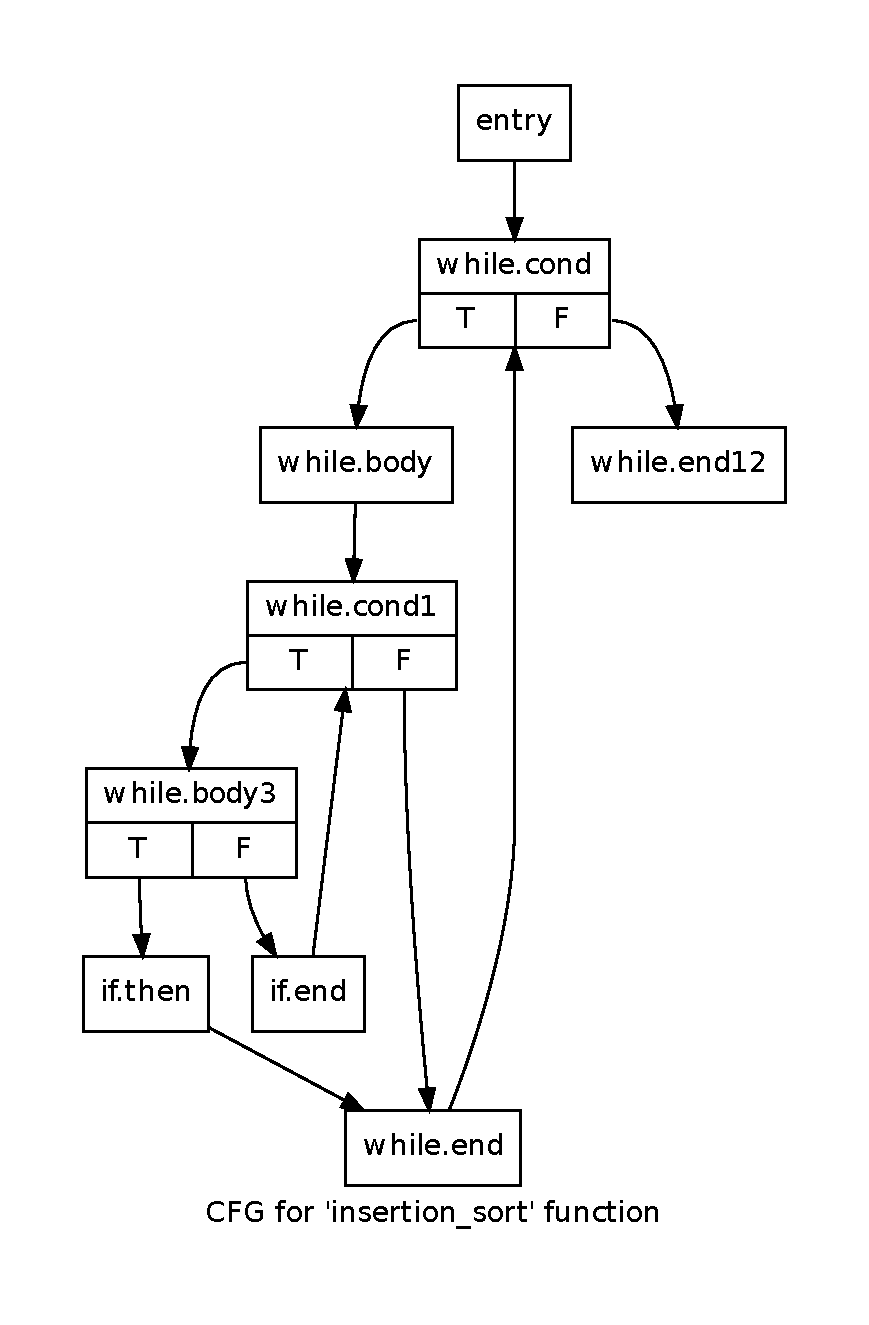
\includegraphics[width=0.90\linewidth]{../assignment/cfg_insertion_sort}
  \end{minipage}%
  \begin{minipage}[c]{.3\linewidth}
    %\vspace{0pt}
    \centering
    \small
    \begin{tabular}{|l|r|}
      \hline
      Basic Block & Cost \\
      \hline
      entry & 12 \\
      while.cond & 6 \\
      while.body & 15 \\
      while.cond1 & 4 \\
      while.body3 & 11 \\
      if.then & 1 \\
      if.end & 21 \\
      while.end & 16 \\
      while.end12 & 1 \\
      \hline
    \end{tabular}
  \end{minipage}
  \caption{Control-Flow Graph for \texttt{insertion\_sort} (from LLVM IR)
           and costs for the execution of basic blocks.}
  \label{fig:cfg.insertion_sort}
\end{figure}

\clearpage
